\documentclass[graybox]{svmult}
\usepackage[T1]{fontenc}
\usepackage{amsmath,amssymb,booktabs,tabularx,graphicx}
\usepackage[numbers,sort&compress]{natbib}
% Preserve the Springer class's smaller reference text after natbib loads.
\renewcommand{\bibfont}{\small}
\usepackage{xurl}
\usepackage[hidelinks]{hyperref}
\pdfstringdefDisableCommands{\def\and{, }}
\makeatletter\let\tableinput\@@input\makeatother
\graphicspath{{figures/}}
\begin{document}
\title*{Online Property Discussion and Dubai Property Sales: An Auditable X--Reddit Study}
\titlerunning{Online Discussion and Dubai Property Sales}
\author{Muath Al Rammal* \and Milan Dordevic \and Nourch\`ene Elleuch Ben Ayed \and Aaron Saji Abraham \and Prajwal Kokatnur}
\authorrunning{Muath Al Rammal et al.}
\institute{\parbox[t]{\linewidth}{\raggedright Muath Al Rammal*, Milan Dordevic, Aaron Saji Abraham and Prajwal Kokatnur \at School of Computer Science, University of Wollongong in Dubai, Dubai, United Arab Emirates. \mbox{\email{muath@uow.edu.au}}*; \mbox{\email{mdordevic@uow.edu.au}}; \mbox{\email{aaronab006@gmail.com}}; \mbox{\email{peterkokatnur26@gmail.com}}.
\and Nourch\`ene Elleuch Ben Ayed \at Higher Colleges of Technology, Dubai, United Arab Emirates. \mbox{\email{nbenayed@hct.ac.ae}}.\\
ORCIDs, in author order: \href{https://orcid.org/0000-0002-3240-6262}{0000-0002-3240-6262}; \href{https://orcid.org/0000-0002-1478-8367}{0000-0002-1478-8367}; \href{https://orcid.org/0000-0002-1155-2471}{0000-0002-1155-2471}; \href{https://orcid.org/0009-0009-0289-5729}{0009-0009-0289-5729}; \href{https://orcid.org/0009-0000-8841-394X}{0009-0000-8841-394X}.\\
*Corresponding author: Muath Al Rammal, \mbox{\email{muath@uow.edu.au}}.}}
\maketitle
% Keep the template's running-head style without its first-even-page box mark.
\makeatletter
\def\@evenhead{\runheadsize\runheadstyle\hbox to\textwidth{\thepage\hfil Muath Al Rammal et al.}}
\makeatother

% Generated by final_corpus_refit/write_paper_numbers.py
\newcommand{\TruncatedTexts}{2,922}
\newcommand{\PrimaryTopics}{367}
\newcommand{\AssignedTexts}{32,561}
\newcommand{\NoiseTexts}{35,724}
\newcommand{\AlternativeTopicRange}{239--425}
\newcommand{\ActivityNoise}{36,592}
\newcommand{\GeoAny}{5,132}
\newcommand{\GeoAnyPercent}{7.54}
\newcommand{\GeoSingle}{4,184}
\newcommand{\GeoSinglePercent}{6.15}
\newcommand{\GeoCells}{145}
\newcommand{\GeoCompleteCells}{15}
\newcommand{\JVCMentions}{1,133}
\newcommand{\SingleLargest}{31,322}
\newcommand{\AverageLargest}{10,540}
\newcommand{\CompleteLargest}{7,923}
\newcommand{\WardLargest}{5,134}
\newcommand{\CompleteGroups}{189}
\newcommand{\CompleteDiameter}{0.449}
\newcommand{\AverageGroups}{165}
\newcommand{\AverageDiameter}{0.652}
\newcommand{\NativeTopics}{147}


\abstract{Linking online property discussion to market activity requires careful data preparation. We combine X, Reddit and Dubai Land Department records in a traceable dataset: 71,239 retained social records dated January--April 2026 (UTC) and 62,012 sales registrations dated January--April 2026 (Dubai time). Source records, cleaning decisions and available conversation context are preserved. An earlier two-reviewer assessment of 400 records provides data-quality evidence. BERTopic fitted to 68,285 unique texts produces 367 topics. LLM semantic labelling supports 43 candidate Specific Market Discourse Indicators (SMDIs), with ten broader groups organised by the authors. Assignments cover 48.6\% of social records. \textbf{TODO: Insert independent SMDI-validation result.} Over 16 complete weeks, Reddit developer and political/social discussion have different relationships with registered sales; X shows different patterns. Several relationships weaken under weekly changes, narrower categories or reduced thread influence. The study contributes a documented dataset and an exploratory comparison of online discussion with sales activity. It does not establish causal effects or forecasting ability.}
\keywords{Real estate; Social media; BERTopic; Discourse measurement; Reproducibility}

\section{Introduction and Related Work}
Social networks can influence housing beliefs and decisions \cite{bailey2018}. Online discussion may show which market issues attract attention. However, more posts do not necessarily mean that more investors hold a view: participation, data collection and labelling also affect the result.

We study January--April 2026 X, Reddit and Dubai Land Department (DLD) records, covering a period that includes the U.S.--Iran conflict \cite{crs2026}. Our contributions are a traceable dataset and an exploratory comparison with sales registrations. We ask:
\textbf{RQ1}: How can the three sources be combined and organised into useful discussion categories?
\textbf{RQ2}: How do weekly discussion shares relate to registered sales and sale amounts?
\textbf{RQ3}: How do the findings change across platforms, off-plan and ready sales, short time lags and different calculation choices?

Earlier housing research has used Twitter language for prediction \cite{zamani} and social-media text to measure sentiment \cite{housing2023}. Economic text indices also show how language can be linked to clearly defined concepts \cite{baker2016}. Our predecessor, \emph{Detecting the Digital Footprint of Speculation} \cite{speculation}, used DLD features to classify transactions. This study instead compares aggregate discussion with market records. It does not identify speculative purchases.

BERTopic groups similar texts \cite{bertopic}, but a cluster is not automatically a meaningful economic category. Automated quality scores may differ from human interpretation \cite{hoyle}, and merging topics changes their level of detail \cite{janssens}. We therefore separate topic discovery from labelling and grouping, drawing on content-analysis and topic-labelling research \cite{hsieh2005,topicgpt}. The final categories still require validation for this particular use \cite{grimmer2013}.

\section{Dataset Construction and Quality Checks}
\subsection{Sources and cleaning}
The snapshots contain 88,155 distinct platform-typed IDs. X combines 12,423 strict-search records and 3,190 accepted broad-search records; a 2,471-ID overlap leaves 13,142. Supporting files track inclusion and exclusion.

Reddit includes r/dubairealestate and selected threads from r/dubai. Its r/dubai filter scores 10,834 of 21,292 submissions after excluding 10,458 deleted bodies, retaining 825 at threshold $>0.4$. Neither source captures all discussion.

We preserve IDs, original/cleaned text, timestamps and available conversation context. X Snowflake timestamps reproduce saved dates. Relevance uses property language in the target or reply context; parent labels are not automatically transferred. Rules remove deleted/empty text, AutoModerator, solicitations and reactions. Scripts document normalisation. X uses English metadata; Reddit language and generic automation flags lack independent validation.

Inspection during development removed 2,064 contact, reaction and promotional records from an initial 74,303 retained records. A later target-text rule removed another 1,000 offers or invitations, while protecting buying questions. Table~\ref{tab:flow} gives the final counts. The primary topic model and five alternatives were fitted after these changes.

\begin{table}[t]
\caption{Dataset counts. Social activity records are distinct source IDs; text families are the units used to fit the topic model.}\label{tab:flow}
\centering\small
\begin{tabular}{lr}\toprule
Population & Count\\\midrule
Social source snapshots & 88,155\\
Initially retained social records & 74,303\\
Additional exclusions: first / second repair & 2,064 / 1,000\\
Final retained social records & 71,239\\
\quad X posts / Reddit submissions / Reddit comments & 11,787 / 4,450 / 55,002\\
Unique text families used for topic fitting & 68,285\\
Common 16 weeks: X / Reddit records & 11,362 / 56,721\\
DLD January--April sales: off-plan / ready & 41,499 / 20,513\\
DLD common 16-week sales & 59,229\\\bottomrule
\end{tabular}
\end{table}

Different IDs remain separate activity records even when text repeats. Topic fitting uses each case-insensitive cleaned-text family's earliest retained record. A near-duplicate check uses five-word sequences, a 20-word minimum and verified Jaccard similarity of at least 0.85. The earlier 74,303-record corpus yielded 358 accepted pairs; 308 retain both endpoints in the final corpus. Sensitivity weights inherit the earlier family grouping. This is a partial check on repetition, not complete detection of copied content.

\subsection{What the existing human review establishes}
The earlier review contains 400 paired records: 99 X posts, 33 submissions and 268 comments. Reviewers disagree on at least one criterion for 57 records (Table~\ref{tab:human}) \cite{cohen1960}. Of the 373 records retained in the final dataset, reviewers 1/2 mark 31/33 as promotional and 32/37 as low-information. Conversely, 10/8 of the 27 excluded records pass all criteria. These findings show remaining cleaning errors. They do not measure the accuracy of the final SMDI categories.

\begin{table}[t]
\caption{Earlier data-quality review ($n=400$). YY/NN mean that both reviewers answered yes/no; YN/NY show disagreements. These questions concern data quality, not SMDI labels.}\label{tab:human}
\centering\small\setlength{\tabcolsep}{4pt}
\begin{tabular}{lrrrrr}\toprule
Criterion & YY & NN & YN & NY & $\kappa$\\\midrule
\tableinput{tables/annotation.tex}
\bottomrule\end{tabular}
\end{table}

On 500 development posts with 33 positive examples, the r/dubai filter has precision 0.719, recall 0.697, F1 0.708 and accuracy 0.962. Always choosing the negative class would give accuracy 0.934. DeBERTa-v3-large zeroshot-v2.0 used the first 1,024 characters; its exact model revision was not recorded.

The final data flag 4,177 possible promotions, 10,386 short contextual records and 45 non-Latin-script records. Root/parent text is missing for 393/366 comments. We test exclusions for promotion and short-context flags; missing context and uncertain language remain limitations.

\section{Building the SMDIs}
\subsection{Topic discovery}
We represent the 68,285 unique target texts using normalised 384-dimensional all-MiniLM-L6-v2 embeddings \cite{sbert,minilmcheckpoint}, reused after checking the pinned model revision, exact text and row order. The encoder's 256-token limit truncates \TruncatedTexts{} texts. Parent text is available for interpretation but is not added to each reply's embedding.

BERTopic 0.17.4 uses UMAP \cite{umap} with 30 neighbours, five dimensions, cosine distance, minimum distance zero and seed 42. HDBSCAN \cite{hdbscan} uses Euclidean distance, excess-of-mass selection, minimum cluster size 20 and minimum samples 10. Topic keywords use one- and two-word terms after removing English stop words, with minimum document frequency two. The model produces \PrimaryTopics{} topics containing \AssignedTexts{} unique texts. Another \NoiseTexts{} texts receive topic $-1$: the model does not place them in a topic. This does not mean that their content is irrelevant.

Alternative cluster size and minimum sample settings (20/5, 40/10, 40/5) and seeds 17/73 produce \AlternativeTopicRange{} topics. We also compare hierarchical merging methods \cite{scipy}. Forcing 25 groups puts \SingleLargest{} of \AssignedTexts{} assigned texts into the largest single-linkage group, compared with \AverageLargest{} for average linkage and \CompleteLargest{} for complete linkage. Complete linkage at cosine-distance 0.45 gives \CompleteGroups{} groups; BERTopic's automatic reduction gives \NativeTopics{} \cite{reduction}. These checks show how grouping choices change the structure. They do not define the SMDIs, and DLD correlations were not used to select them. \emph{Clustering organises the evidence; researchers define the discussion categories.}

\subsection{Labelling topics and forming broader groups}
Each topic's review packet contains keywords, size and representative posts. According to the authors, GPT 5.6 Sol provided semantic labels. The workbook preserves the labels and mapping, but the complete original prompting session is not archived and cannot be regenerated exactly. It contains 43 candidate \emph{Specific Market Discourse Indicators} (SMDIs), with one finer-category assignment per topic. The workbook flags 309 topics as clear, 48 as interactional/discourse and ten as mixed/manual-check. These are development judgments, not independent validation results.

The authors then manually organised the topics into ten broader groups (Table~\ref{tab:coverage}). These groups overlap and sometimes divide a finer category between groups. We therefore keep two explicit mappings: topic-to-SMDI and topic-to-broad-group. All 367 topics are included, but this is not a simple hierarchy in which each finer category belongs wholly to one broad group.

A record receives the labels of its topic. If $z_i$ is record $i$'s topic and $T_g$ contains the topics in group $g$, then
\begin{equation}
a_{ig}=\mathbf{1}(z_i\in T_g)\mathbf{1}(z_i\ne-1).\label{eq:assignment}
\end{equation}
A record counts once per group and can appear in several groups. There is no extra keyword rule or separate document classifier. Mixed topics can give unsuitable record labels; topic $-1$ remains unassigned.

The group names are broader than individual economic concepts. Political/geopolitical/social discussion includes reactions and humour, while developers/projects includes reputation and launches. We test narrower existing categories as well. The main analysis uses Pass 1 only; later experiments on unassigned texts remain in the development files and do not change these indicators.

\subsection{Independent SMDI validation}
\textbf{TODO: Independent SMDI validation.} Two reviewers will label a stratified sample without seeing assignments or DLD results. Cover finer categories, overlaps, mixed topics, platforms, periods and unassigned records. Report agreement before adjudication, category precision/recall where estimable, and missed content. The earlier 400-record review does not supply category labels.

\section{Market Data and Comparisons}
The DLD export contains 105,466 rows, including 171 exact duplicates. After removing these, sales account for 80,882 rows but 80,868 registration IDs. Repeated sales IDs agree on the transaction fields and differ only in nearby-place information, so they are counted once. We do not apply this rule to mortgage or gift records.

January--April contains 62,012 sales registrations: 41,499 off-plan and 20,513 ready. Their total recorded amount is AED 224.952 billion, with a median of AED 1.719 million. These are amounts attached to registrations, not a price index that holds property quality constant. DLD also distinguishes the area transacted from the full property area \cite{dlddata}.

We use 16 complete Monday--Sunday weeks in Dubai time, from 5 January to 26 April. They contain 68,083 social records and 59,229 sales registrations worth AED 215.323 billion. Partial weeks are excluded, including 38 social records dated 1 May locally but 30 April UTC. A registration date does not reveal when the buyer made the decision.

For group $g$, platform $p$ and week $t$, we calculate
\begin{equation}
S_{gpt}=\frac{\sum_{i\in(p,t)}a_{ig}}{N_{pt}},\qquad
S^{A}_{gpt}=\frac{\sum_{i\in(p,t)}a_{ig}}{N^{A}_{pt}}.\label{eq:smdi}
\end{equation}
$N_{pt}$ is the number of all retained platform records that week; $N^A_{pt}$ counts only records assigned to a topic. The main measure $S$ is the proportion of all records identified with the group. The alternative $S^A$ describes only topic-assigned records. Their relationship, $S=S^A(N^A/N)$, shows how topic coverage affects the result. Neither tells us the unknown category membership of unassigned records. X and Reddit are kept separate; likes and other engagement counts are not weights.

The main analysis has four comparisons for each platform: market/pricing (G1) against median sale amount; developers/projects (G3) against off-plan and ready counts; and political/geopolitical/social discussion (G9) against all sales counts. Other group plots provide context. Sales counts do not directly measure rents, legal disputes, living conditions or platform behaviour.

We compare discussion with sales in the same week and one or two weeks later. These comparisons have 16, 15 and 14 pairs respectively. We report Pearson and Spearman correlations, changes from the previous week, results after removing a linear trend, and results after leaving out each week in turn. Since earlier project results were known, this is an exploratory analysis rather than a preregistered test.

Related weeks complicate correlations \cite{rankcorrelation}. A paired stationary bootstrap \cite{bootstrap} resamples aligned blocks of discussion and sales (4,999 repetitions; average lengths 2/3/4). Its intervals depend on the resampling assumptions and exclude category-labelling errors; nominal 95\% coverage is not established for this 16-week sample.

Checks use counts, alternative denominators, repetition and author/thread weights, quality-flag exclusions, UTC weeks and two-week periods. Period medians are recalculated from registrations. Mean amounts and median flat amounts per transacted square metre check transaction composition. SMDI-03 (valuation), SMDI-27 (off-plan/delivery) and SMDI-14 (geopolitical conflict) test narrower meanings.

\section{Results}
\subsection{How much discussion receives a label?}
All 34,647 topic-assigned activity records receive a finer category and at least one broad-group label. This is 48.6\% of 71,239 records; 3,930 belong to more than one broad group. Another 36,592 records remain unassigned. Topic coverage is 5,350/11,787 (45.4\%) on X and 29,297/59,452 (49.3\%) on Reddit. Across the 16 weeks, it ranges from 38.0\% to 59.7\% on X and 46.3\% to 52.1\% on Reddit. Coverage is not an accuracy measure.

\begin{table}[t]
\caption{Broad-group coverage. Counts are activity records; percentages use all retained X ($N=11,787$) or Reddit ($N=59,452$) records. Groups overlap.}\label{tab:coverage}
\centering\small\setlength{\tabcolsep}{3pt}
\begin{tabular}{lrrr}\toprule
Group & Topics & X $n$ (\%) & Reddit $n$ (\%)\\\midrule
\tableinput{tables/domain_coverage.tex}
\bottomrule\end{tabular}
\end{table}

Market/pricing and developer discussion take larger shares on X. Locations, services and tenancy take larger shares on Reddit (Table~\ref{tab:coverage}). These differences describe the collected data, not all users of the platforms. \textbf{TODO: Add independent SMDI-validation results by platform and period.}

\subsection{Discussion and sales in the same week}
Figure~\ref{fig:weekly} compares movement by subtracting each series' average and dividing by its standard deviation. The lines show relative changes, not absolute sizes. Table~\ref{tab:primary} uses the original shares and values.

\begin{figure}[p]\centering
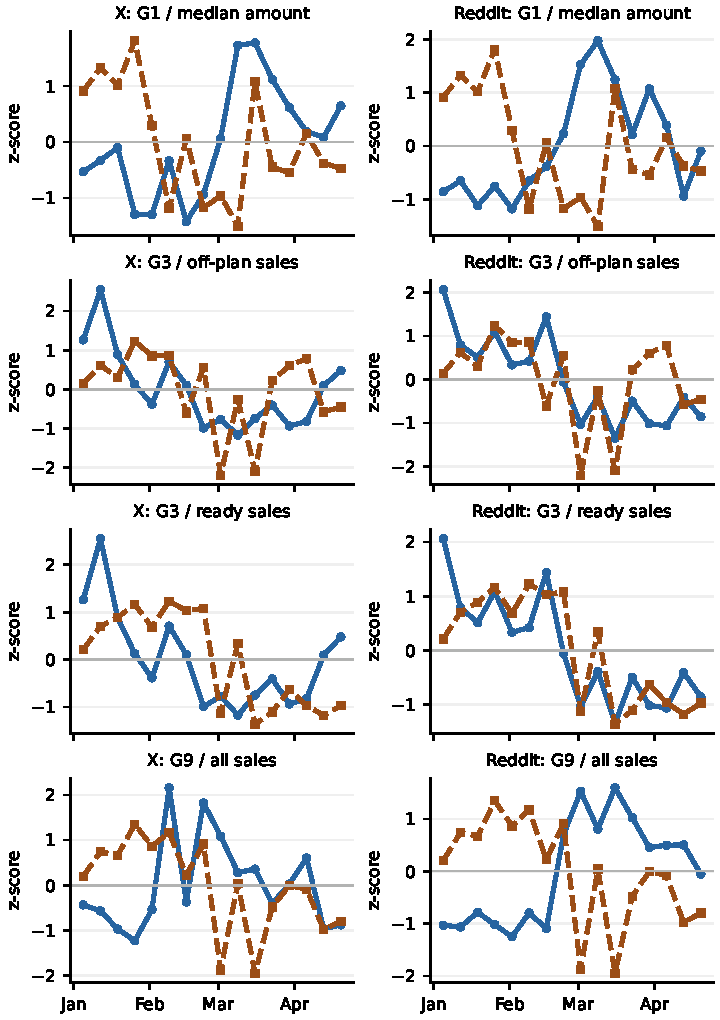
\includegraphics[width=\textwidth]{domain_comparisons.pdf}
\caption{Direct comparisons over 16 complete weeks. Blue: the group's share of all retained platform records. Dashed: the specified DLD measure. Each series is shown relative to its own average in standard-deviation units. G1: market/pricing; G3: developers/projects; G9: political/geopolitical/social discussion. X and Reddit are shown separately.}\label{fig:weekly}
\end{figure}

\begin{table}[t]
\caption{Same-week comparisons ($n=16$). $r$: Pearson; $\rho$: Spearman; $r_\Delta$: correlation of weekly changes ($n=15$). Intervals use the paired bootstrap (95\%, average block length 3).}\label{tab:primary}
\centering\small\setlength{\tabcolsep}{3pt}
\begin{tabular}{lllrrrr}\toprule
Platform & Group & DLD measure & $r$ & $\rho$ & $r_\Delta$ & Interval\\\midrule
\tableinput{tables/domain_correlations.tex}
\bottomrule\end{tabular}
\end{table}

On Reddit, a larger market/pricing share tends to occur in weeks with a lower median sale amount ($r=-0.49$). However, the correlation between their weekly changes is almost zero ($-0.01$). The relationship therefore does not describe a consistent week-by-week movement.

Reddit developer discussion has a stronger relationship with ready-sale counts ($r=0.75$) than off-plan counts ($r=0.42$). Correlations of weekly changes are lower, at $0.38$ and $0.22$. The X relationships are weaker and turn negative when we examine weekly changes.

Reddit political/geopolitical/social discussion has a negative relationship with sales counts ($r=-0.76$), weakening to $-0.42$ for weekly changes. X has almost no same-week relationship ($r=-0.01$). Since this group includes general reactions and controversial discussion, the Reddit result is not a measure of geopolitical risk alone.


\subsection{Do the findings change under other choices?}
The main Reddit relationships change little when percentages use only topic-assigned records. Giving threads equal weight within each week reduces pricing versus amount to $-0.30$, developers versus ready sales to $0.64$, and political/social discussion versus sales to $-0.61$. One thread contributes up to 30.1\% of weekly political/social records.

Narrower categories give different findings. Reddit's off-plan/delivery category correlates $-0.19$ with off-plan counts and $0.11$ with ready counts, compared with $0.42$ and $0.75$ for the broad developer group. There are no X records in this finer category during the common period, so its correlations cannot be calculated. The narrower geopolitical-conflict category gives $-0.68$ for Reddit sales and $-0.27$ for X. The narrower Reddit valuation category gives $-0.40$ with median sale amount. These changes show why the exact category meaning matters.

Changing the market measure also matters: Reddit pricing gives $-0.26$ with median flat amount per transacted square metre, versus $-0.49$ with median sale amount. Neither is a constant-quality price index. Removing a linear trend reduces the X pricing relationship to approximately zero.

Later-sales comparisons do not give a consistent leading signal. Reddit developer/ready correlations are $0.72$ and $0.64$ at one- and two-week lags, but weekly-change correlations are approximately zero and $-0.36$. X reaches $0.67$ at both lags, falling to $0.35$ and approximately zero for weekly changes. All lag results are provided in the supporting files.


\subsection{Can we compare neighbourhoods?}
Among the 68,083 common-period records, exact DLD-area names match \GeoAny{} (\GeoAnyPercent{}\%); \GeoSingle{} (\GeoSinglePercent{}\%) have one match. Of \GeoCells{} platform--area combinations, only \GeoCompleteCells{} cover every week. JVC appears in \JVCMentions{} records without a validated DLD mapping. Mentions do not locate authors or transactions, so we do not calculate neighbourhood correlations.

\section{Discussion and Conclusion}
The dataset makes posts, cleaning decisions, context and sales records traceable. Earlier human review reveals remaining cleaning errors. The 43 categories and ten broad groups offer different detail, but over half of activity remains unassigned and mixed topics can give unsuitable record labels.

Reddit's developer and political/social groups relate differently to sales. Weekly changes and narrower categories weaken several results; broad developer findings do not establish delivery-related findings. Combining platforms would also hide differences.

Changing information conditions provide varied discussion, not independent label validation or evidence of an event's market effect. Sixteen weeks cannot separate lasting relationships from shared shocks, capture changes or registration delays. \textbf{TODO: Update the interpretation after independent SMDI validation.} Nonrepresentative capture, residual promotions, truncation and missing edit histories limit generalisation.

The accompanying \nolinkurl{research_companion.zip} contains the codebook, topic mappings, weekly aggregates, result tables and reproduction scripts. Its documentation follows established dataset and computational reporting practices \cite{datasheets,wilson}. Aggregate checks need no raw posts. Full reconstruction requires restricted data and embeddings; saved scores and labels preserve inputs whose original generation cannot be repeated exactly. Private text, identities, reviews and models are excluded.

\bibliographystyle{spmpsci}
\bibliography{references}
\end{document}
